\chapter{样式}

\section{转义字符}
注意“\#\,”是 \TeX 元字符,因此 C\# 要写作 \fn{C\bs\#}。
类似的“\textasciitilde”也是元字符,
要写作\mn{textasciitilde}。
\index{命令!textasciitilde@\mn{textasciitilde}}
这两个字符在URL中也经常出现,要特别小心。

C/C++代码的标识符中经常出现下划线“_”,例如 \fn{boost::shared_ptr}、
\fn{random_\linebreak[0]shuffle} 等。
为了避免每次都转义,可以使用 \fn{underscore} 宏包,
将下划线变为普通字符。
\index{宏包!underscore@\fn{underscore}}
注意这里 \fn{random_\linebreak[0]shuffle} 在行尾断字,
那么下划线之后不应该出现连字号“-”,
因此应写为 \verb|random_\linebreak[0]shuffle|。

\section{斜体}
按照排版规范,数学变量名和(非标准)函数名应该用斜体,
常量、单位、标准函数名应该用正体。
例如:%$\footnote{c是真空中的光速,k是Boltzmann常数。}:
$n$-body 问题、%$E = m \mathrm{c}^2 、
%$V_\mathrm{T} = \frac{\mathrm{k} T}{q}$、
$\sin x = (\mathrm{e}^{\mathrm{i}x} - \mathrm{e}^{-\mathrm{i}x})/2\mathrm{i}$、
5\textmu s。
快速排序 $n$ 个元素的数度的平均时间复杂度是 $O(n \log n)$。
通过 TCP 发送 $n$ 字节的消息,
接收方收到这 $n$ 个字节的事件可能性有 $2^{n-1}$ 种
\footnote{在 $n-1$ 个字节间隙中,依次插入 $0, 1, \ldots, n-1$ 个“隔板”,
一共有 $C_{n-1}^0 + C_{n-1}^1 + \cdots + C_{n-1}^{n-1} = 2 ^ {n-1} $ 种情况。}。

\section{列表}
\LaTeX 默认的列表环境(\fn{itemize} 和 \fn{enumerate})是为多行文字准备的,
因此上下间距较大。我一般使用 \fn{enumitem} 宏包来重新定义列表环境,
并且定义几个简单的命令来使用它(\mn{begindot} 和 \mn{myenddot},\mn{beginnum} 和 \mn{myendnum})。
\index{宏包!enumitem@\fn{enumitem}}
\begin{Code}
\newcommand\begindot{\begin{itemize}
[itemsep=2pt plus 2pt minus 2pt,%
topsep=3pt plus 2pt minus 2pt,%
parsep=0pt plus 2pt minus 2pt]}
\newcommand\myenddot{\end{itemize}}
\end{Code}

\begin{Code}
\newcommand\beginnum{\begin{enumerate}
[itemsep=2pt plus 2pt minus 2pt,%
topsep=3pt plus 2pt minus 2pt,%
parsep=0pt plus 2pt minus 2pt]}
\newcommand\myendnum{\end{enumerate}}
\end{Code}

\section{章节标题}
章节标题无标点,因此 \S \ref{sec:whyTypesetting} 是错的。
\fn{ctex} 宏包默认会把章\mn{chapter} 和节\mn{section} 的标题居中,
这种样式显得很古板,章标题可以靠右,节标题和小节标题均靠左。
参见本文的\fn{format.cls} 文件。

\subsection{编号}
通常单个小节不编号,因此 \S \ref{subsec:noChineseItalic} 和本小节是错的。
应要改用\mn{subsection*} 命令。

\section{图表编号} %%%%%%%%%%%%%%%%%%%%%%%%%%%%%%

我不使用浮动环境,因此自己定义了 \mn{figcaption} 和 \mn{tabcaption} 命令来为图表编号。
图的标题位于下方,按章编号(图1-1、图1-2、图2-1 等等)。
例如

\begin{center}
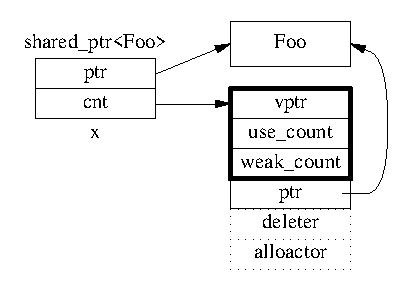
\includegraphics{sp0.eps}\\
\figcaption{\fn{shared_ptr} 的数据结构}\label{fig:sharedptr}
\end{center}


表的标题位于上方,按章编号(表1-1、表1-2、表2-1 等等)。
例如

\begin{center}
\tabcaption{水平空格命令的长度}

\vspace{1ex}
\begin{tabular}{ccl}
\hline
\textbf{命令} & \textbf{长度} & \textbf{用途}\\
\hline
\mn{quad} & 10pt & 图表编号与图表标题之间的全角空格\\
\mn{,} & 1.67pt & 千分空,例如 65\,536\\
\hline
\end{tabular}
\end{center}

\section{脚注} %%%%%%%%%%%%%%%%%%%%%%%%%%%%%%

\subsection{编号}
\LaTeX默认是按章重置脚注编号,
这么如果重印的时候需要增加一个脚注,
势必会影响后续页码,这是 \mybooktitle 排版的一个教训。
因此我意识到脚注应该是按页重置,但是 \verb|\@addtoreset{footnote}{page}|
无效,必须使用 \fn{footmisc} 宏包的 \fn{perpage} 选项,
例如 \sfn{\bs usepackage[perpage]\{footmisc\}}。
\index{宏包!footmisc@\fn{footmisc}}

\LaTeX默认的脚注编号是数字,这有时会造成误解。
例如给长度单位pt添加脚注,正文中可能会出现“pt\textsuperscript{2}”,
让人误以为是面积单位,因此可以改用带圈数字。

\subsection{置底}
\LaTeX默认的脚注位置不是固定置底,而有可能随页面内容而浮动。例如 \myurl{footnote-middle.tex}。

\vspace{1ex}
\centerline{\fbox{
\includegraphics[page=1]{footnote-middle.pdf}}%
\quad\fbox{
\includegraphics[page=2]{footnote-middle.pdf}}}

使用 \fn{footmisc} 宏包的 \fn{bottom} 选项之后,
脚注置底。见 \myurl{footnote-bottom.tex}。 \nopagebreak

\vspace{1ex}
\centerline{\fbox{
\includegraphics[page=1]{footnote-bottom.pdf}}%
\quad\fbox{
\includegraphics[page=2]{footnote-bottom.pdf}}}

\section{参考文献}
技术书籍不是学术著作,可不必使用 BibTeX 工具,直接按出版社的格式要求排版参考文献即可。
